\chapter{Centralized control of the offloading infrastructure}
\label{cha:vehicular-offloading-service}

In this chapter, we propose an architecture  that leverage the advantages of the logical centralization provided by SDN\index{Software Defined Networking (SDN)|)} to enable efficient control of the road infrastructure to offload bulk delay-tolerant data from an infrastructure network. SDN provides the logistics including planning, implementing, and controlling for the effective and efficient transportation of data over the road network.  

%Our offloading service relies on private vehicles equipped with storage devices combined with the use of offloading spots which refer to wireless data storage devices located where vehicles park as part of their line of travel. Figure~\ref{fig:taxonomy} gives an overview of the operations involved in the offloading of large amounts of delay-tolerant background data over the road network between two remote data centers. We target long-lived data transfers lasting several days to a few weeks. These transfers result from provisioning or maintenance activities across remote data center sites, typically required for virtual machine migrations or offline backups. 

%As a result of the data transfer allocation, the offloaded data follows the allocated paths traveled by the vehicles on the roads connecting the successive offloading spots involved in the data transfers. 

We propose a centralized architecture for flexible and scalable configuration of the network of offloading spots. We use the SDN (\textit{Software-Defined Networking}) paradigm, which provides the logistics for efficient and effective vehicular transportation of data. Our SDN-controlled architecture consists of a central controller and a collection of offloading spots. 
%The controller receives demands to offload data transfers onto the road network. An offloading demand indicates the source and destination of the transfer as well as its performance requirements (\eg in terms of delay and bandwidth). 
The controller is in charge of mapping a data transfer onto a sequence of offloading spots matching the direction of a vehicle against the destination of the data.

To enable efficient data offloading, our architecture needs to be designed so to cope with the high degree of complexity of the road network topology and the large number of daily routine journeys involving vehicles. This lead us to propose a road map reduction procedure which produces a logical representation of the road network infrastructure. This representation will be used as an input for the data transfer allocation procedure presented in Chapters~\ref{cha:feasibility-study} and~\ref{chap:implementation}. Each formulate the allocation procedure problem according to two linear programming (LP) models that maximizes the cost benefits that result from using vehicles as data carriers and maximizes the road traffic utilization, respectively. 
%Updates of allocation decisions are also required for maintaining high utilization in face of changes in the road traffic.

%Firstly, our architecture needs to have a global view of the flows of vehicles so to efficiently assign them the data transfers. The offloading spots then use the output of the allocation to decide which data to load or unload from the stopping vehicles. Secondly, this architecture must be scalable to make the data transfer allocation problem tractable. To this end, it must mitigate the complexity of the road network topology and the large number of vehicular trips.

Our main contributions in this chapter are the following two:
\begin{itemize}

    \item \textbf{Centralized architecture.} We present a centralized architecture that enables scalable and adaptive control of the road network to offload traffic. This architecture also provides the control to guarantee reliable data transfers.
    
    \item \textbf{Road map reduction.} We propose a mapping algorithm which produces an  offloading overlay, a logical representation that characterizes the movements of the vehicles into network quantities. The offloading overlay mitigates the complexity of the road network and makes the data transfer allocation problem tractable.
    
    %\item {\bf Road network resource allocation.} We design an allocation procedure that selects vehicle flows to match the performance requirements of offloading demands.
    	
\end{itemize}

This chapter is structured as follows. In Section~\ref{sec:overview-service}, we present an overview of our offloading service by introducing the reference scenario we will use throughout the thesis. In Section~\ref{sec:offloading-system-operations}, we present a centralized architecture that draws on the SDN paradigm to enable scalable and adaptive control the road network infrastructure. In Section~\ref{sec:offloading-service-model}, we give an abstract model of the offloading service by which we introduce the notations we will use in the rest of this document. In Section~\ref{sec:mapping-offloading-overlay}, we introduce an algorithm for reducing the complexity of the road network. The output of our algorithm is an \textit{offloading overlay} which gives a logical representation of the road network. The offloading overlay allows us to propose models to allocate data transfers onto the road network.

\begin{figure}[h!]
	\centering
		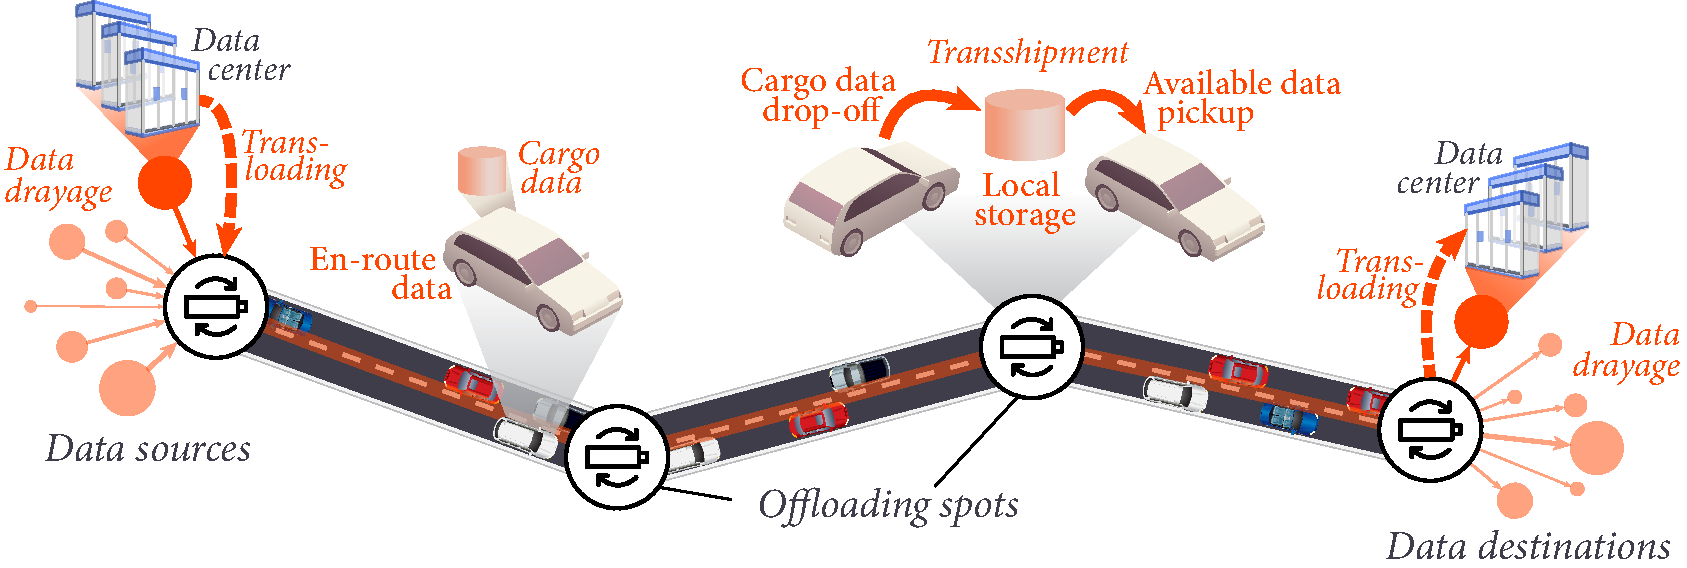
\includegraphics[width=0.75\columnwidth]{figures/taxonomy.pdf}
	\caption{Overview of our road-based offloading service.}
% 	Part or all the data of a transfer between two remote data centers is shifted from the Internet to the road network. Data is first transloaded by means of drayage to the closest edge offloading spot until transferred on empty stopping vehicles. Subsequent intermediate offloading spots act as data relays where vehicles can drop off data on their route for later pick-up and delivery by other vehicles. Once at destination, the data is transloaded back into the data network.}
	\label{fig:taxonomy}
\end{figure}

\section{10,000-foot view of the offloading service}
\label{sec:overview-service}



The decision of loading data on or off vehicles is taken by the offloading spots according to forwarding states installed by an SDN-like controller. The offloading spots act similarly to forwarding engines under the direct authority of the controller. The next section describes the SDN centralized architecture we propose for efficient data offloading onto the road network.   

%The offloading spots act as data exchange relays to compose the trajectories of vehicles traveling in different directions. 
 
%We take advantage of the parking time to opportunistically load on or unload data from vehicles while they are stopped at the offloading spots. The data is \textit{transloaded}\index{transloading} from a conventional data network to the closest offloading spot by means of \textit{drayage}\index{drayage}. 

%The data is stored until transferred to stopping vehicles that will carry it to its destination.

%The offloading service provider\index{offloading service provider|bb}, if different from the vehicle manufacturers, offers a ``get paid to drive'' program to the vehicle owners. The service provider installs the storage devices and the vehicle owners\index{vehicle owner} receives a monthly fee or a discount on the cost of refilling or charging their vehicle in exchange for driving their normal routine. The discount rate is negotiated with the gas station operator\index{gas station operator} (\eg Total or BP) in the case of internal combustion engine vehicles or the charging station operator\index{charging station operator} (\eg ChargePoint or Tesla) in the case of electric vehicles\index{Tesla}. The discount rate is calculated based on the driving pattern including coverage and mileage. If the vehicle manufacturers take on the role of service provider, vehicles are equipped as standard with on-board storage devices and the offloading service is provided without involving nor compensating the vehicles' owners. The service provider charges the content provider\index{content provider} for the amount of data to offload on the road network and shares the revenues with the gas or charging station operator\index{charging station operator}.


\section{Centralized controlled offloading architecture}
\label{sec:offloading-system-operations}

We leverage the advantages of the logical centralization provided by \acrfull{sdn}\index{Software-Defined Networking (SDN)} to enable efficient control and management of the road network resources to offload bulk delay-tolerant traffic from a conventional data network. Following \acrshort{sdn}'s original design, our architecture consists of two components, as depicted in Figure~\ref{fig:architecture}: a central controller\index{controller} and the offloading spots acting as forwarding entities. We describe the function of each component in the remainder of this section and evaluate the benefits of the central controller in Section~\ref{sec:need-for-controller}. 

\begin{figure}[t]
	\centering
	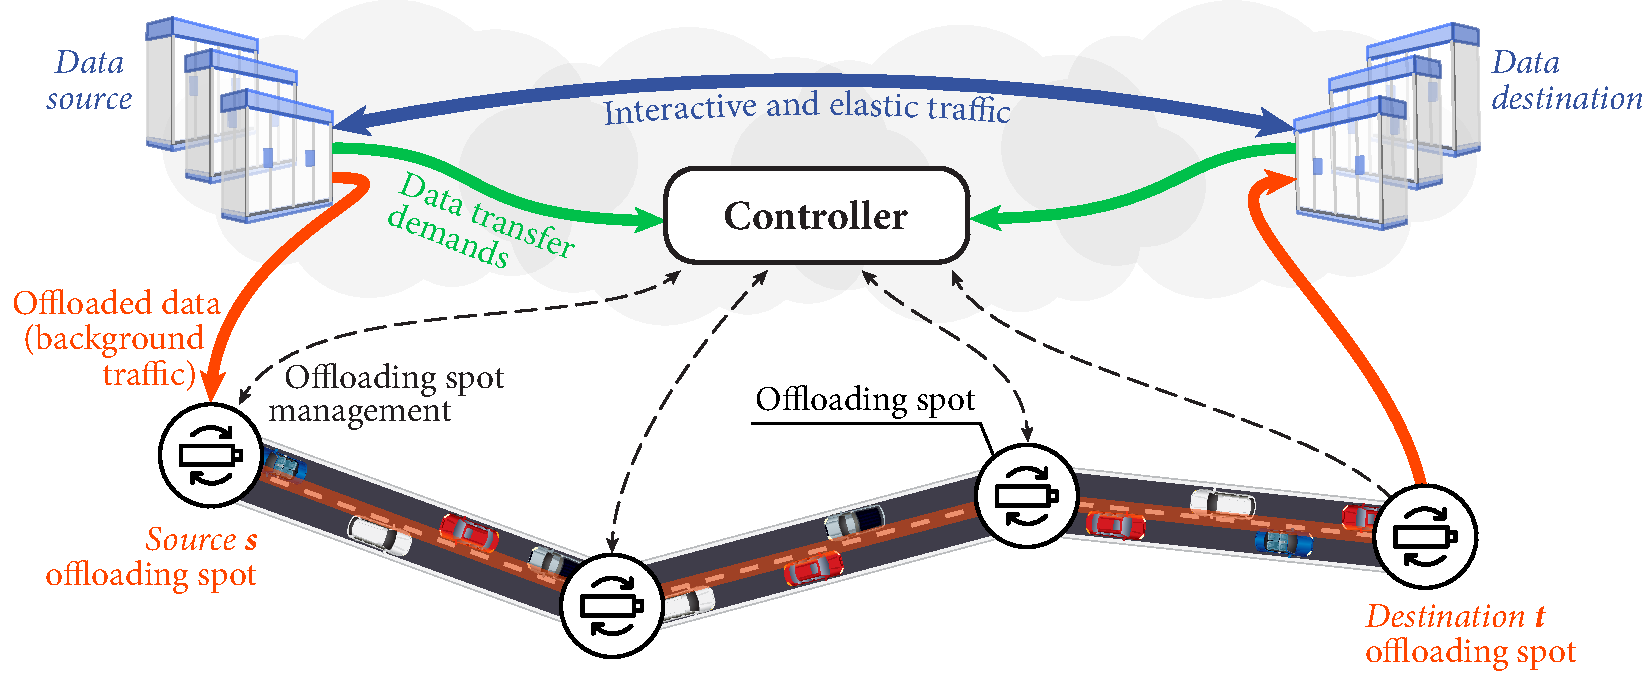
\includegraphics[width=0.75\columnwidth]{figures/architecture2.pdf}
	\caption{Centralized architecture for the offloading service.}
% 	In this scenario, the controller receives demands to offload bulk transfers of delay-tolerant data between two data centers. The controller configures the road network data plane by installing forwarding states at the offloading spots. The controller allocates the flows of vehicles on the roads connecting the offloading spots to carry the data towards its destination.}
	\label{fig:architecture}
\end{figure}

\subsection{Controller}

The controller\index{controller|bb} has a holistic knowledge of the road network including its topology and dynamics, such as the traffic volumes for each road segment. Such knowledge may be derived from traffic forecasting services such as Navteq/Here\footnote{\url{https://www.here.com/business/traffic}},     
TomTom\footnote{\url{http://automotive.tomtom.com/en/connected-services/tomtom-traffic}}, or 
Airsage.\footnote{\url{http://www.airsage.com/Products/Traffic-Insights/}}. The controller keeps track of the status of the offloading spots via a long range control channel (\eg SIGFOX\footnote{\url{http://www.sigfox.com/}}). The information about the offloading spots includes the metadata of the data in transshipment and the statistics about the stopping vehicles, including the historical locations' made available via the navigation system of the vehicles. By collecting the information about the offloading spots, the controller has an up-to-date view of the offloading system. In Section~\ref{sec:discuss}, we present a list of probabilistic tools for inferring the remaining route of a vehicle knowing its navigation history.       

The controller receives demands\index{offloading demand} to offload data from transfers on the road network. Each demand specifies the delay and bandwidth requirements for the corresponding data transfer, as well as the origin and destination. When receiving an offloading demand, the controller selects the road network paths by solving the data transfer allocation problem\index{data transfer allocation problem}. A road network path consists of a sequence of offloading spots followed by the data carried by vehicles between the offloading spots. We formulate the data transfer allocation problem as two linear programming (LP) models. A first one is the revenue maximization problem we present and solve in Chapter~\ref{cha:feasibility-study}. A second one formulates the allocation as the throughput maximization problem in Chapter~\ref{chap:implementation}. In both models, the data transfer allocation problem determines the road networks path and also how much data to allocate to the flows of vehicles traveling between the consecutive offloading spots along the road network paths. 

Figure~\ref{fig:controller-flowchart} shows the interactions between the functions of the controller with those of the offloading spots. The allocation procedure involves a reduction of the road network with the offloading overlay we detail in the next section. 

\begin{figure}[t]
	\centering
		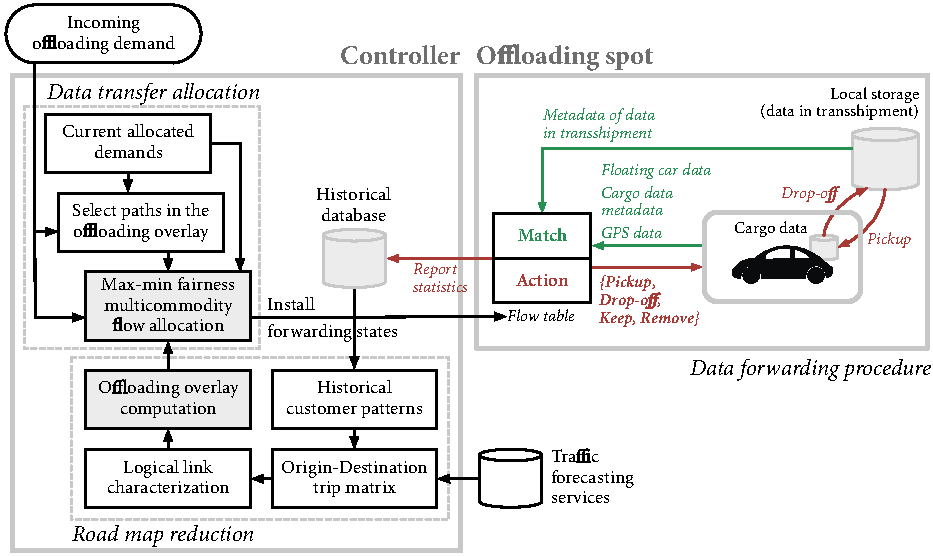
\includegraphics[width=\columnwidth]{figures/controller-flowchart-offloading-spot.pdf}
	\caption{Interactions between the functions of the controller and those of the offloading spots.}
	\label{fig:controller-flowchart}
\end{figure}


\subsection{Data forwarding at the offloading spots}
\label{sec:data-forwarding-offloading-spot}

We represent the interactions between the actions of the controller and the offloading spots in Figure~\ref{fig:controller-flowchart}. The controller installs forwarding states to control the local decisions made at the offloading spots to either drop off or pick up the data cargo. This decision results from the matching of the direction of the stopping vehicles against the destination of the available data. The local decisions account for the allocation of the road network resources shared among concurrent offloaded data transfers.

\begin{wrapfigure}[24]{o}[0.7\marginparwidth]{7.6cm}
    \includegraphics[width=7.5cm]{figures/forwarding.pdf}
    \caption{Forwarding process at an offloading spot.}
    \label{fig:forwarding-process}
\end{wrapfigure}
\paragraph{Flow tables.} 
The forwarding behavior of an offloading spot is determined by its \textit{flow table}\index{flow table|bb} represented in Figure~\ref{fig:controller-flowchart}. It consists of a list of entries, each installed for an individual offloading demands. The controller adds a new entry in the flow table of all the offloading spots on the road network path resulting from the allocation of a data transfer.
A flow entry contains the next-hop offloading spot to forward the data car along the allocated road path toward its destination.
% A flow entry forwards the data cargo to the next-hop offloading along the computed road path toward its destination.
% A flow table entry contains the next-hop offloading spot to which the data must be forwarded to reach the destination of the data transfer corresponding to this entry. 
The destination of the stopping vehicles is matched against the next-hop offloading spot of the flow entries. If there is a match, the offloading spot performs an action described by the forwarding process.
% on the cargo carried by the vehicle associated with the entry, including loading data on or off the vehicles.

\paragraph{Forwarding process.} 
The forwarding process is represented by the flowchart depicted in Figure~\ref{fig:forwarding-process}. Upon the arrival of a vehicle, an offloading spot checks if the direction of the vehicle matches one entry of its flow table. If none of the entries match, the vehicle unloads, if any, its data cargo onto the offloading spot storage for future pick-ups and continues its journey without performing any further actions. If multiple entries match the direction of an empty vehicle, the offloading spot selects one entry based on the scheduling strategies presented in Section~\ref{sec:scheduling}. After selecting one of the entries, the offloading spot performs the actions specified in the entry. If the vehicle already carries data, the offloading spot checks if this data belongs to the data transfer represented by the matching entry. If this is the case, the vehicle keeps its cargo and continues its journey. Otherwise, the vehicle unloads its cargo at the offloading spots before resuming its journey. In case the vehicle arrives empty, if some data matching the vehicle direction is locally available, the data is transferred to the vehicle. Otherwise, the vehicle continues its journey without a cargo. 

\subsection{Evaluating the benefits of a centralized control}
\label{sec:need-for-controller}

To assess the benefits of a central controller, we use a simple scenario composed of four offloading spots as depicted in Figure~\ref{fig:simple-scenario}. We compare different scheduling strategies when concurrent data transfers traverse an offloading spot. Two data transfers $A$ and $B$ originate from offloading spot $S$ and share the road segment connecting offloading spot $I$. The transfers then follow their route toward their final destinations $T_A$ and $T_B$, respectively. 
We only consider the road traffic on the road segments shown in the figure.


\begin{figure}[ht]
    \centering
    \begin{subfigure}[t]{0.4\columnwidth}
        \centering
        % \raisebox{.2\textwidth}{
        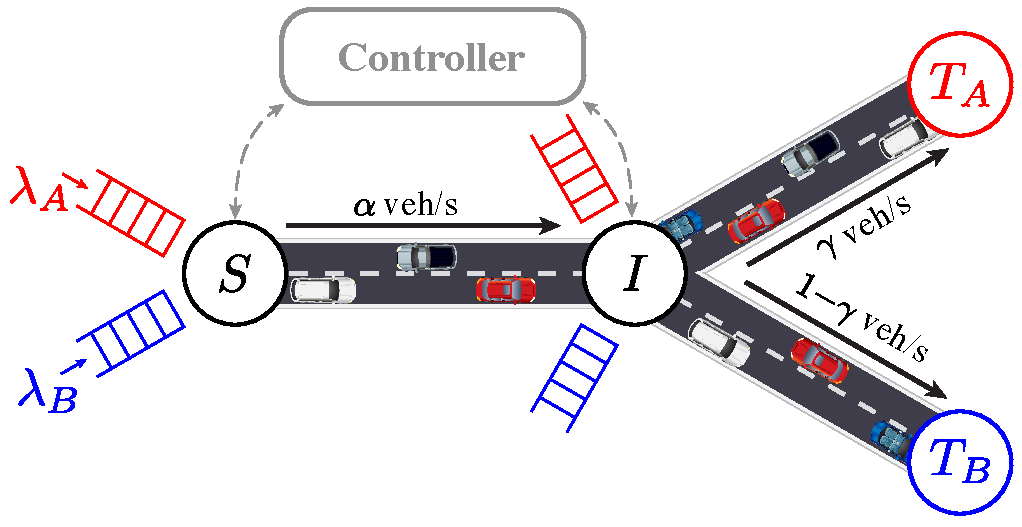
\includegraphics[width=\textwidth]{figures/simpleScenario.pdf}
        % }
        \caption{Two data transfers $A$ and $B$ originating from offloading spot $S$ share the road connecting offloading spot $I$. They then follow their own route toward their final destinations $T_A$ and $T_B$, respectively.}
        \label{fig:simple-scenario}
    \end{subfigure}%
    \quad %add desired spacing between images, e. g. ~, \quad, \qquad etc.
      %(or a blank line to force the subfigure onto a new line)
    \begin{subfigure}[t]{0.47\columnwidth}
        \centering
        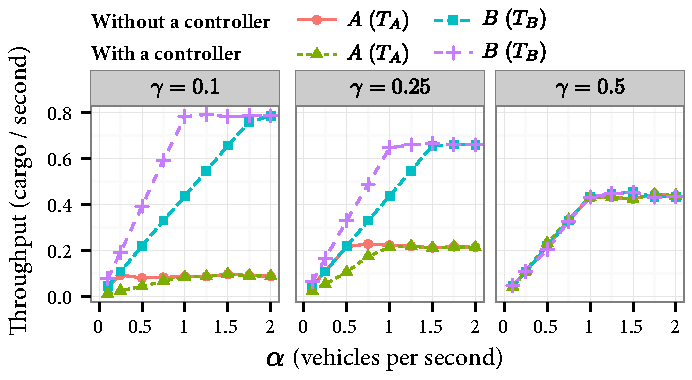
\includegraphics[width=\textwidth]{results/simpleScenario-throughput_v2_gamma.pdf}
        \caption{Maximum throughput (in number of data cargo received per second), for the two strategies with and without controller as a function of parameters $(\alpha,\,\gamma)$.}
        % (deduced from the AADT values)
        \label{fig:simple-scenario-throughput}
    \end{subfigure}
    \caption{Road network consisting of four offloading spots to show the benefits of having a controller.}
\end{figure}

We consider two scheduling strategies, without a controller and with a controller, to select the data transfer and to determine the amount of data to load on the vehicles stopping at each offloading spot. The first scheduling strategy (without a controller) selects the data cargo available at the offloading spots in a round-robin fashion. The data cargo of the transfers is selected in equal proportions and in circular order, without any priority given to the transfers. In the second strategy (with a controller), the decision to load a cargo on a vehicle is based on forwarding states installed at the offloading spots. The controller determines the forwarding states using the traffic volumes of road network under consideration. In the example of Figure~\ref{fig:simple-scenario}, if we assume the road traffic volume $I\rightarrow T_A$ to be three times greater than $I\rightarrow T_B$, the second strategy (with a controller) will load data three times more often onto vehicles heading to $T_A$. This is not the case of the strategy without a controller: this strategy will load the same amounts of data on stopping vehicles regardless of whether they head to $T_A$ or $T_B$.

We use \acrshort{sumo} (\acrlong{sumo})~\cite{behrisch2011sumo} to evaluate the three scheduling policies and simulate microscopic traffic in volumes of $\alpha$ vehicles per second from $S$ to $I$, $\gamma$ from $I$ to $T_A$, and $1 - \gamma$ from $I$ to $T_B$. We assume that both transfers $A$ and $B$ have infinite backlog of data at offloading spot $S$ (\ie $\lambda_A = \lambda_B = \infty$). Figure~\ref{fig:simple-scenario-throughput} shows the throughput of the system measured in the number of data cargo delivered to the destinations per second. In the scenario, the scheduling is relevant at $S$, as the road segments connecting the next-hop offloading spot $I$ to $T_A$ and $T_B$ exhibit different road traffic volumes. We consider an infinite backlog traffic generated at $S$ such that all vehicles leaving offloading spot $I$ are loaded with a cargo.

We can see that, for the first strategy without a controller, the transfer headed to $T_A$ needs a longer ramp-up period to reach its nominal throughput. Without any knowledge on the downstream traffic volumes, $S$ cannot load the optimal amounts of data to the next offloading spot $I$ to fully utilize the network resources. As a result, $I$ does not have enough data locally available to feed the higher flow of vehicles traveling towards $T_B$ compared to destination $T_A$. The resources available on the road segment $(I,\,B)$ remain underused when not enough data belonging to transfer $B$ are transported in an adequate amount to offloading spot $I$, \eg for $\alpha = 2$. On the contrary, the second strategy with controller allows $S$ to load data on vehicles traveling to $I$ in adequate amounts for both transfers. In turn, $I$ has enough data to efficiently utilize vehicles traveling on towards $T_A$ as well as $T_B$. The controller leverages the knowledge of traffic volumes on the downstream road segments to maximize the use of road resources at offloading spot $S$. This second strategy can achieve a better throughput performance for all competing transfers at $I$. 


\section{Road map reduction}
\label{sec:offloading-service-model}

In this section, we present a mapping algorithm that reduces the complexity of the road network. The output of our algorithm is an offloading overlay\index{offloading overlay|bb}, which refers to a logical representation that captures the characteristics and dynamics of the road network. We provide a performance evaluation that measures the reduction factor resulting from the mapping algorithm by comparing the complexity of the offloading overlay over the actual road network.

\subsection{Road network}
\label{sec:road-network-characterization}

We represent the road network\index{road network|bb} by a directed graph $G^R=(N^R,\,L^R)$, where $N^R$ and $L^R$ denote the set of physical nodes and links, respectively. The set of nodes $N^R=N^J\cup N^S$ consists of two subsets: the set of road junctions ($N^J$) and the set of charging stations ($N^S$). A road junction refers to a location where vehicles can change their direction of travel. A link in the road network corresponds to a road segment connecting two adjacent junctions or a junction and a charging station. We consider the road segments and the traffic flowing in both directions homogeneous as they share the same profile in terms of capacity and free-flow speed. For a road segment $(a,\,b)\in L^{R}$, let $v_{ab}$ be its nominal volume of vehicles (vehicles per unit of time), $c_{ab}$ be its capacity (vehicles per unit of time), and $t_{ab}(0)$ be its corresponding travel time at free-flow speed (\ie when $v_{ab}=0$). 

\subsection{Offloading overlay}
\label{sec:offloading-overlay-characterization}

The offloading overlay\index{offloading overlay|bb} provides a logical view\index{logical view} of the road network. More specifically, the overlay mitigates the combinatorial explosion when enumerating the simple road paths in the road network, which becomes
\begin{wrapfigure}[14]{o}[0.7\marginparwidth]{7.5cm}
    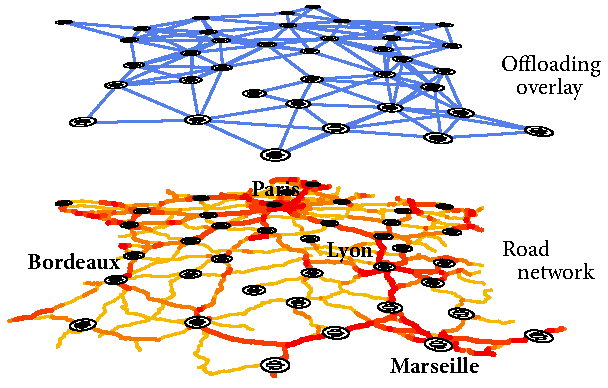
\includegraphics[width=7cm]{figures/France-overlay-1.pdf}
    \caption{The offloading overlay resulting from the deployment plan of offloading spots for the French road network in Section~\ref{sec:charging-station-network} (the width and darkness of the road segments denote the vehicle density).}
    \label{fig:France-overlay}
\end{wrapfigure}
quickly intractable. By providing a logical view\index{logical view} of the vehicle movements on the road paths connecting the offloading spots, the offloading reduces the number of paths to enumerate. 
%and makes the data transfer allocation problem tractable.

We represent the offloading overlay by a directed graph $G^O=(N^O,\,L^O)$, where $N^{O}$ and $L^{O}$ denote the set of logical nodes and links, respectively. A logical node of $N^{O}$ is an offloading spot. A logical link of $L^{O}$ represents the road path (\ie a sequence of road segments) connecting two adjacent offloading spots in the road network. Note that multiple road paths may connect two adjacent offloading spots. In Figure~\ref{fig:France-overlay}, we show an example of realization of an offloading overlay on top of the French road network. 

In the following Section~\ref{sec:characterization-offloading-overlay}, we characterize a logical link $(i,\,j)\in L^{O}$ with network quantities, that is by the weighted travel time $t(i,\,j)$, aggregated capacity $c(i,\,j)$ and data leakage $l(i,\,j)$. The data leakage refers to the loss rate on logical link $(i,\,j)\in L^{O}$ and accounts for the proportion of vehicles that fail to deliver the data to the next offloading spot $j$ because of errors in the prediction of the direction of the vehicle or accidents. We assume that offloading spots are not constrained by the amount of transfers they can serve and have the adequate storage capacity so that the overall service is stable. 
%We evaluate the benefits of the offloading overlay over the raw road network in Section~\ref{sec:complexity-offloading-overlay}. 

\subsection{Mapping algorithm}
\label{sec:mapping-offloading-overlay}

In this section, we present the algorithm we use to map the offloading overlay. We use publicly available datasets with \acrfull{aadt}\index{AADT} for the road segments to characterize the logical links with network quantities. \Acrshort{aadt} is the total volume of traffic traveling on a road segment in both directions for one year, divided by the number of days in the year. The algorithm relies on transportation forecasting\index{transportation forecasting|bb} techniques to translate the traffic counts for the road segments into traffic volumes traveling between the offloading spots. The algorithm proceeds in the steps detailed in the following sections.

\subsubsection{Route determination}
\label{sec:route-determination}

\begin{wrapfigure}[13]{o}[0.4\marginparwidth]{5.5cm}
    \vspace{-10pt}\resizebox{0.9\linewidth}{!}{\begin{tikzpicture}[node distance=2cm]
	\tikzset{
	    bigN/.style={draw,circle,minimum width=0.3cm,inner sep=0},
	    smallN/.style={draw,circle,minimum width=0.3cm,inner sep=0} 
	}
	\node[bigN] (1) at (0,0) {} 
		node[smallN,fill=red] at (1.center) {}
		node at (1.south) [below] {$S$};
	\node[smallN] (3) at (1.5,0.65) {};
	\node[smallN] (2) at (2,-1) {};
	\node[smallN] (4) at (3,-0.5) {};
	\node[smallN] (5) at (3.5,0.25) {};
	\node[smallN] (6) at (4.5,-1.5) {};
	\node[smallN] (7) at (5,1) {};
	
	\node[smallN,dashed] (8)  at (6,2.5) {};
	\node[smallN,dashed] (9) at (6,-1.7) {};
	\node[smallN,dashed] (10) at (7,0.5) {};
	
	\draw (1) -- (2);
	\draw (1) -- (3);
	\draw (1) -- (4);
	\draw (1) -- (5);
	\draw[thick] (1) -- (6);
	\draw[thick] (1) -- (7);
	
	\fill[pattern=custom north west lines,hatchcolor=red] 
		  (-30:5cm) -- (-30:5.5cm)
	      arc (-30:30:5.5cm) -- (30:4.5cm)
	      arc (30:-30:4.5cm) -- cycle;
	\fill[red] 
		  (-30:5.5cm) -- (-30:6cm)
	      arc (-30:30:6cm) -- (30:5.5cm)
	      arc (30:-30:5.5cm) -- cycle;
	\draw[red] (1) -- (-30:6cm) 
		node [pos=0.82,below,sloped] {\textit{refill}};
	\draw[red] (1) -- (30:6cm)
			node [pos=0.4,above,sloped] {Range of the vehicle}
			node [pos=0.98,above,sloped] {\textit{critical}};
	\node[anchor=base west] at ($(-30:6cm) +(0:0.2cm)$) {\textit{Out-of reach}};
\end{tikzpicture}}
\vspace{-5pt}
    \caption{Illustration of the range of a vehicle and the offloading spots within its range.}
    \label{fig:vehicle-range}
\end{wrapfigure}

The first step\index{transportation forecasting!route determination} consists of selecting a subset of the alternative routes connecting each pair of adjacent offloading spots in the road network. Adjacent offloading spots are those within a pre-defined range of the vehicles as shown in Figure~\ref{fig:vehicle-range}. In the case of electric vehicles, the range is limited to the autonomy of the battery. Current electric vehicles have an autonomy of 300~km on average (\eg up to 473~km for the Tesla Model S 90D\footnote{\url{https://www.Teslamotors.com/models}}, 210~km for the Renault Zoe\footnote{\url{http://www.renault.fr/gamme-renault/vehicules-electriques/zoe}}, and 180~km for the Nissan LEAF\footnote{\url{http://www.nissanusa.com/electric-cars/leaf/charging-range/}}). In the case of internal combustion engine\index{internal combustion engine} vehicles, the range is generally higher than electric vehicles. Note that the range of the vehicles highly depends on the driving behavior of the drivers. In the simulations of the following chapters, we considered a conservative vehicle range of 300~km.

The selection of the road paths consists in choosing the paths that are the most relevant to the behavior of the drivers. A natural approach to this problem is to use the All-or-Nothing assignment, which assigns the road traffic to the shortest route between two points~\cite{dijkstra1959note,delling2009engineering,hart1968formal}. While the shortest route may be used by most of the drivers, it does not account for the alternative routes chosen by other drivers, in the case of congestion or road work for instance. To determine multiple routes, on can use algorithms that compute the $k$-shortest routes in terms of travel time~\cite{yen1971finding,eppstein1998finding}. However, for large networks, these algorithms yield routes that are most of the time not reasonable and not actually used by the drivers. More recent algorithms try to determine the most reasonable alternative routes between two points~\cite{geisberger2010route,abraham2013alternative}. In the evaluations of Chapter~\ref{chap:implementation}, we use the algorithm proposed by Abraham \etal~\cite{abraham2013alternative} to determine the most reasonable alternative routes in the road network of France. With this algorithm, the routes are selected such that they share a low degree of similarity in terms of road segments in common. 

\subsubsection{Route assignment}
\label{sec:route-assignment}

The second step\index{transportation forecasting!route assignment} consists in assigning weights to the selected routes. The weights give the proportion of traffic $p(k)$ that will use a certain route $k$. If only one route $k$ was selected by a shortest-path algorithm, then, all the road traffic is assigned to this route and $p(k) = 1$. However, if a set of road paths were selected in the route determination step, we determine the proportion of traffic to assign to each selected route using route choice and traffic assignment strategies. These strategies determine weights to the selected routes. The values of the weights are determined according to attributes such as the travel time and the distance of the routes. 
\begin{wrapfigure}[15]{o}[0.7\marginparwidth]{7.5cm}
    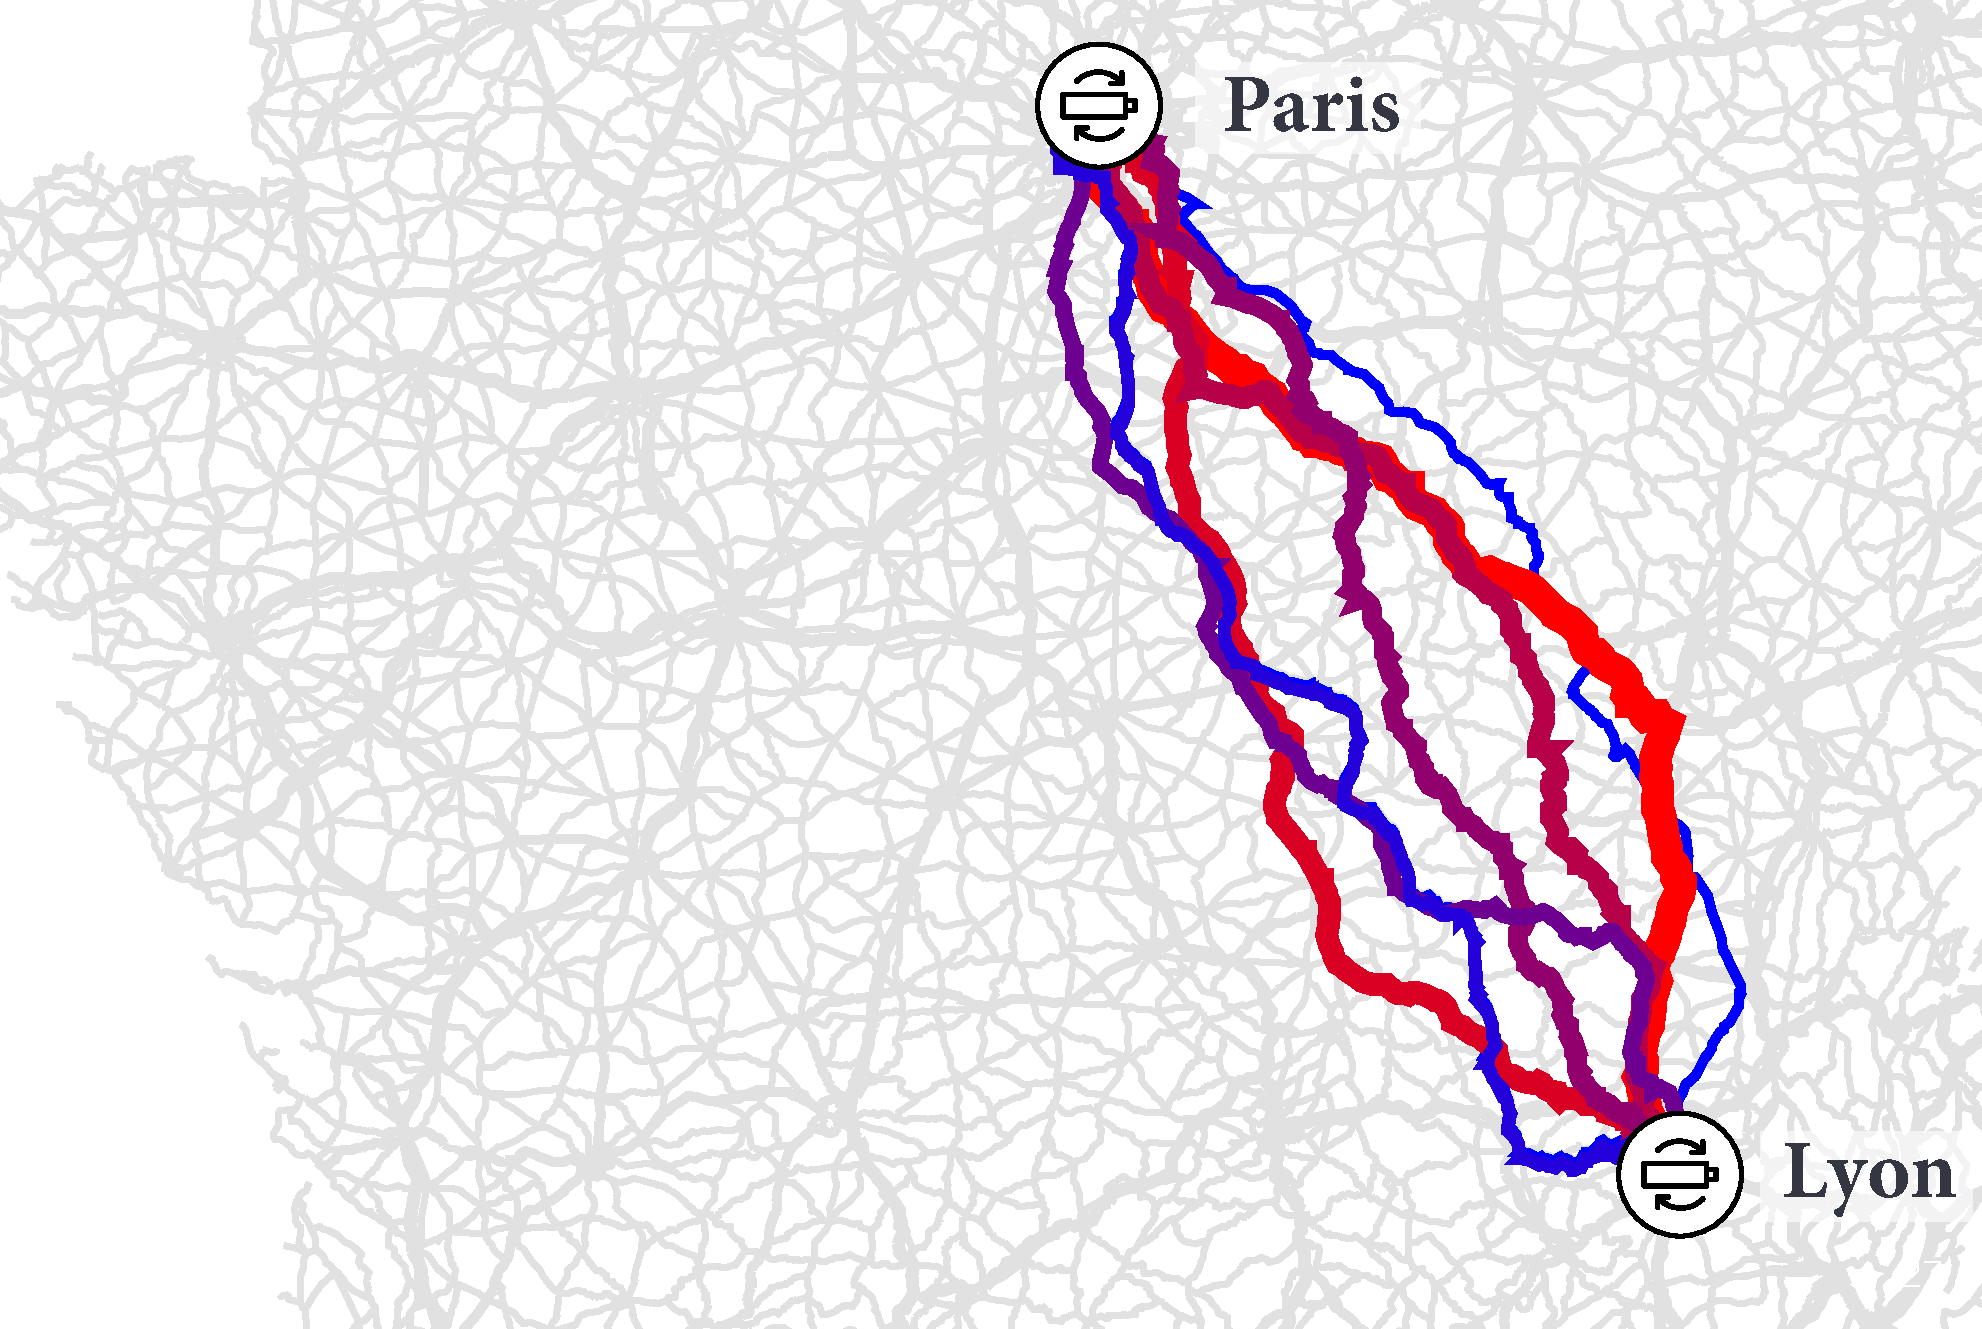
\includegraphics[width=7cm]{figures/route-assignment.pdf}
    \caption{Top 10 routes between Paris and Lyon chosen by the algorithm proposed by Abraham \textit{et al.}~\cite{abraham2013alternative}. The red thickest route is the shortest path and the width of the routes depends on the weights assigned to the routes by the C-Logit traffic assignment~\cite{cascetta1996modified}.}
    \label{fig:route-assignment}
\end{wrapfigure}
Those weights reflect the capacity of a route in attracting traffic, the higher the weight of a route, the more traffic it will receive. To this end, stochastic-user-equilibrium (S-U-E) techniques~\cite{daganzo1977stochastic} were derived from the user-equilibration criterion formulated by Wardrop~\cite{wardrop1952some}. The user-equilibration criterion specifies the following two principles:
\begin{enumerate}
    \item In an equilibrated network, users cannot improve their travel time by changing routes.
    \item The average journey time of all drivers is at a minimum.
\end{enumerate}
The S-U-E techniques build on Wardrop's principles to propose stochastic route assignment algorithms. These techniques include Dial's or C-Logit stochastic traffic assignments~\cite{dial1971probabilistic,cascetta1996modified}.  In the evaluations of Chapter~\ref{chap:implementation}, we use the C-logit route assignment model~\cite{cascetta1996modified} to determine the weights on the selected routes in the road network of France. The C-Logit traffic assignment is a multinominal logit model that assigns a choice probability $p(k)$ on a path $k$ using a perceived utility $U_k$ to each path $k$ of the selected paths:
\begin{equation}
U_k = V_k + \varepsilon_k\quad \forall k,
\end{equation}
where $V_k$ is the average or systematic utility of path $k$ (\eg distance or travel time) and $\varepsilon_k$ is the random residual that includes perception errors of the user’s decisions. Here, we consider the utility $V_k$ is the sum of the inverse of the travel time of each road segment in the road path $k$.

The choice probability, or weight, $p(k)$ for path $k$ is expressed as:
\begin{equation}
p\left(k\right)=\frac{\exp\left[V_{k}-CF_{k}\right]}{\sum_{h\in\mathcal{{P}}^{st}}\exp\left[V_{h}-CF_{h}\right]}\Comma
\end{equation}
where the term $CF_{k}$ is the ``commonality factor'' of path $k$, which is directly proportional to the degree of similarity of path $k$ with the other selected paths. Here, we consider the following expression of the commonality factor:
\begin{equation}
CF_{k}=\beta_{0}\ln\sum_{h\in\mathcal{P}^{st}}\left(\frac{L_{hk}}{L_{k}^{1/2}L_{h}^{1/2}}\right)^{\gamma}\Comma
\end{equation}
where $L_{hk}$ is the length of common paths to $h$ and $k$, $L_{h}$ and $L_{k}$ are the lengths of paths $h$ and $k$, respectively, and $\gamma$ is a positive parameter. Typically, $\beta_{0} = 1$ and $\gamma = 1$ or $\gamma = 2$~\cite{cascetta1996modified}.

The weights determined by the traffic assignment techniques are then used in combination with the traffic counts to estimate the traffic volume of the routes selected in the first step between each pair of adjacent offloading spots. 


\subsubsection{Trip matrix estimation}
\label{sec:trip-matrix-estimation}

In the third step\index{transportation forecasting!trip matrix estimation}, we determine the origin-destination trip matrix that characterizes the number of trips between each pair of adjacent offloading spots. This step can be done qualitatively by conducting travel surveys to know the travel habits of the populations within a geographical area. Examples of these national surveys include the \acrfull{nhts} in the United States\footnote{\url{http://nhts.ornl.gov}} and the \acrfull{entd} in France.\footnote{\url{http://www.statistiques.developpement-durable.gouv.fr/sources-methodes/enquete-nomenclature/1543/139/enquete-nationale-transports-deplacements-entd-2008.html} (in French)} These surveys are conducted by governmental agencies about every ten years. The last version of the \acrshort{nhts} dates from 2009 while the last version of the \acrshort{entd} dates from 2008. There is currently a newer version (2016) of the \acrshort{nhts} survey being conducted. A lower bound of an estimate of the road traffic $T_{ij}$ between pairs of locations $(i,\,j)$ corresponds to the traffic volume $v_{ab}$ of the road segment $(a,\,b)\in L^{R}$ with the lowest traffic of the shortest road path $k$ between the two locations (\ie that corresponds to the bottleneck of the road path). The volume is weighted by $w(d(k))$, the proportion of trips accounted in travel surveys of the same distance as the one of the shortest road path $d(k)$. This estimate can be expressed as follows:
\begin{equation}
    T_{ij} = w(d(k))\times\min_{(a,\,b)\in k}\{v_{ab}\},
\end{equation}

Because these surveys take time and are expensive to conduct, there exist other techniques to estimate traffic matrices between selected locations. These techniques usually rely on \acrfull{aadt}\index{AADT}. It is important to underline that the \acrshort{aadt} is a fundamental statistic used in traffic engineering and transportation planning. The use of the \acrshort{aadt} helps reduce the effects of seasonal bias and missing data mainly due to equipment failure, construction schedules, and installation dates that plague continuous traffic monitoring~\cite{wright1997variability}.

In particular, Zuylen and Willumsen~\cite{van1980most} proposed an entropy-maximizing formulation\index{entropy-maximization problem|bb} to estimate the most likely \acrfull{od} trip matrix\index{origin-destination trip matrix|bb} between the defined locations. The objective of the formulation is to maximize the number of ways of selecting an \acrshort{od} matrix with a total number of trips. As the number of trips increases, the number of ways of selecting an \acrshort{od}  matrix gets more and more peaked and converges to a most likely state. This results in maximizing the entropy of the \acrshort{od}  matrix. The constraint guarantees that the resulting \acrshort{od}  matrix will not overcome the volumes of traffic $v_a$ measured on the road segments $a$. 
\begin{flalign*}
    & \text{Maximize} -\sum_{ij}\big(T_{ij}\log T_{ij} - T_{ij}\big), & \\
    \shortintertext{subject to}
    & v_{a} - \sum_{ij}T_{ij}p^{a}_{ij} = 0 \qquad \forall a \in L^{R}.\\
\end{flalign*}
The probability $p^{a}_{ij}$ denotes the route choice probability of route between source $i$ and destination $j$ to take link $a$ among $S_{ij}$, the set of selected road path. This probability is derived from the choice probability and computed in the route assignment as follows:
\begin{equation}
p^{a}_{ij} = \sum_{\substack{k\in S_{ij}\\k\ni a}} p(k),
\end{equation}
where s.

Since the optimization problem presented above is convex, the authors presented an iterative balancing algorithm to solve it, derive from Bergman's method to solve such problems~\cite{bregman1967proof}. The algorithm is presented in Algorithm~\ref{alg:iterative-balancing}. Each balancing iteration adjusts the quantity $\lambda_{a}$, the road traffic assigned to each road segment $a$. This adjustment is done until all the constraints on the volumes of the road segments are satisfied.
\begin{algorithm}
    \caption{Iterative balancing algorithm for the entropy maximization problem.}
	\DontPrintSemicolon
	\SetKwBlock{Step}{}{}
		
	\Step(\textbf{Step 1.} Initialization){
		$\lambda_{a} \gets 0\quad \forall a\in L$\;
	}	
		
	\BlankLine
	
	\Step(\textbf{Step 2.} Iterative balancing){
		\Repeat{Convergence}{
			$T_{ij}^{\star} \gets \exp\left(\sum_{a}\lambda_{a} \, p^{a}_{ij}\right)\quad \forall i,\,j$\;
			\ForAll{constraints (over domain $L^{R}$)}{
				\If{$V_{a} \neq \sum_{ij}T_{ij}^{\star} \, p^{a}_{ij} $}{
					$\lambda_{a} \gets \lambda_{a} + \ln(V_{a}) - \ln\left(\sum_{ij}T_{ij}^{\star} \, p^{a}_{ij}\right)$
				}
			}
		}
	}
    \label{alg:iterative-balancing}
\end{algorithm}


\subsubsection{Characterization of the offloading overlay} 
\label{sec:characterization-offloading-overlay}

Finally, we characterize the logical links\index{logical link|bb} of the offloading overlay with network quantities, which we determine as follows for each logical link $(i,\,j)$. These network quantities are relevant to solve the data transfer allocation problem.

\paragraph{Travel time $t(i,\,j)$.} 
 The travel time $t{ab}$ of $(a,\,b)$ is given by the \acrfull{bpr} function defined as~\cite{BPR64}:

\begin{equation}
  \label{eq:BPR}
  t_{ab}(v_{ab})=t_{ab}(0)\left[1+\alpha\left(\frac{v_{ab}}{c_{ab}}\right)^{\beta}\right]\Comma
\end{equation}

\noindent where $\alpha$ and $\beta$ are \acrshort{bpr} parameters that depend on the road profile ($\alpha = 0.15$ minutes and $\beta = 4.0$ are typically used)~\cite{HCM00}.

We can deduce from Equation~\ref{eq:BPR} the travel time of physical path $p$, denoted $t_{p}$, which is the sum of all travel times of the road segments that compose the path (we do not consider any turning delays at junctions):

\begin{equation}
  \label{eq:path-delay}
  t_{p} = \sum_{(a,\,b)\in p} t_{ab}(v_{ab}).
\end{equation}

From Equation~\ref{eq:path-delay}, we deduce an expression of the average travel time\index{logical link!average travel time} $t(i,\,j)$ experienced on the $r$ physical paths between nodes $i$ and $j$, weighted by the road traffic flow $v_{p}$ on each path $p$:

\begin{equation}
  \label{eq:ovelray-link-delay}
  t(i,\,j) = \frac{\sum_{p\in S_{ij}} t_{p}\,v_{p}}{r\sum_{p\in S_{ij}}v_{p}}\Comma
\end{equation}

\noindent where $S_{ij}$ is the set of all simple physical paths between $i$ and $j$ (\ie with no cycles in the path).

\paragraph{Capacity $c(i,\,j)$.}
The capacity\index{logical link!capacity} $c(i,\,j)$ of the overlay link $(i,\,j)\in L^{O}$ depends on the sum of the traffic flows $v_{p}$ of the simple paths between offloading spots $i$ and $j$ (\ie the number of vehicles per unit of time going from $i$ to $j$ on path $p$). The capacity $c(i,\,j)$ of the overlay link also depends on the market penetration ratio\index{market penetration ratio|bb} $\mathcal{M}$ of the vehicles participating in the offloading service and the storage size\index{storage size} $\mathcal{S}$ on each vehicle. We assume that all vehicles are equipped with a storage device of the same size $\mathcal{S}$.

\begin{equation}
  c(i,\,j) = \mathcal{M} \times \mathcal{S} \sum_{p\in \mathcal{P}^{ij}} v_{p}.
\end{equation}


\paragraph{Leakage $l(i,\,j)$.}
The leakage\index{logical link!leakage} $l(i,\,j)$ (comprised between 0 and 1) of logical link $(i,\,j)\in L^{O}$ represents the proportion of data that is lost between offloading spots $i$ and $j$. The leakage increases as more vehicles carrying data prematurely exit the road (\eg the vehicles may exit the highway before reaching the offloading spot or an accident may have occurred). The leakage depends on characteristics that are inherent to the physical paths mapped in the offloading overlay. Additionally, the leakage accounts for the errors inherent to the scheduling and forwarding at the offloading spots. In the evaluations of both the feasibility study (Chapter~\ref{cha:feasibility-study}) and the realization (Chapter~\ref{chap:implementation}), we measure the impact of the leakage on the performance of the offloading system. In both of these chapters, we propose different approaches to mitigate the effects of the leakage:
\begin{itemize}
    
    \item In Chapter~\ref{cha:feasibility-study}, we tolerate a target leakage (leakage tolerance) resulting from the successive logical links traversed by the data cargo. To satisfy this tolerance, we consider two replications approaches that load each cargo multiple times on vehicles, either at the source of the data transfers or locally at each intermediate offloading spot involved in the transfer.
    
    \item In Chapter~\ref{chap:implementation}, we use redundancy techniques to decrease the effects of the leakage and retransmission techniques to completely recover the losses due to the leakage. The retransmissions of the lost data cargo are done either at the source of the data transfer or at the intermediate offloading spots.

\end{itemize}

\paragraph{Logical path $p$.}
In the data transfer allocation problems of the following chapters, $p$ denotes a logical simple path\index{logical path|bb} (\ie without any cycles) defined as the ordered list of offloading spots connected by logical links. $\mathcal{P}_{st}$ denotes the set of all logical simple paths from $s$ to $t$. We characterize the logical paths by the travel time $t(p)$ and the flow (throughput) $f(p)$ allocated on logical path $p\in\mathcal{P}_{st}$ for a given offloading demand $d_{st}$ resulting from the data transfer allocation problem. The logical path travel time corresponds to the average time it takes to transfer one data cargo from one extremity of the path to the other. Note that its expression depends on the allocation model we consider.


\subsection{Benefits of the offloading overlay}
\label{sec:benefits-offloading-overlay}

In this section, we evaluate the benefits of the offloading overlay over the raw road network in terms of the number of paths to enumerate between two distant locations. To this end, we consider the road network of France and select offloading spots among a set of suitable candidate locations. We then use real traffic counts measured on the road network of France to build and characterize the corresponding offloading overlay. To be consistent with our motivating scenario, and without loss of generality, we assume that the vehicles are electric vehicles with a range of 300~km. Note that we will use the same dataset throughout the evaluations of Chapters~\ref{cha:feasibility-study} and~\ref{chap:implementation}.

\subsubsection{Dataset of French road traffic}

\begin{wrapfigure}[16]{o}[0.7\marginparwidth]{6cm}
    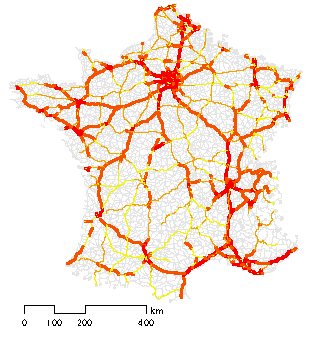
\includegraphics[width=5.7cm]{figures/france-dataset.pdf}
    \caption{Dataset showing the \acrfull{aadt} of the major roads of France in 2011. The road segments have a darker shade when \acrshort{aadt} is higher.}
    \label{fig:france-dataset}
\end{wrapfigure}
Throughout the evaluations we conduct in this thesis, we will use a dataset\index{French road network} collected in 2011 featuring the \acrfull{aadt}\index{AADT} of the major roads in France covering a combined distance of 20,000~km\footnote{\acrshort{entd}~---~Census of the road traffic on the French roads in 2011 (in French): \url{http://tinyurl.com/otfbewv}}.  The traffic volumes are collected using strategically located automatic traffic recorders. The different thickness and shades of red of the road segments depicted in Figure~\ref{fig:france-dataset} reflect the traffic counts given by the \acrshortpl{aadt}. The graph consists of 3,310 edges covering over 20,000~km of roads. 

\subsubsection{Planning of the network of charging stations}
\label{sec:charging-station-network}

We consider a network of charging stations equivalent to the one Tesla\index{Tesla} is currently rolling out in Europe and North America\footnote{\url{https://www.Teslamotors.com/supercharger}}. This network of stations helps electric vehicles face the problem of limited autonomy and achieve long distance travels. Recall that the offloading process will take place in these stations in a transparent manner to the driver. Since there was no such a network in France at the beginning of this thesis, we plan a simple yet realistic network of stations that covers the major roads of France. To plan such a network of stations, we consider a facility-allocation problem\index{facility-allocation problem} that minimizes the number of facilities to allocate, a problem we adapted from the maximal covering location problem~\cite{church1974maximal}. The problem takes demand points and candidate locations as inputs:
\begin{itemize}

	\item The demand points are the 9,555 cities of France with a population greater than 1,000.
   
	\item The candidate locations are the 1,024 Total gas stations, a French oil company.\footnote{\url{http://www.total.fr/mes-deplacements/outils-en-mobilite/export-gps-stations.html} (in French)}

\end{itemize}

\begin{figure}[ht]
    \centering
    \begin{subfigure}[t]{0.4\columnwidth}
            \centering
            % \raisebox{.2\textwidth}{
            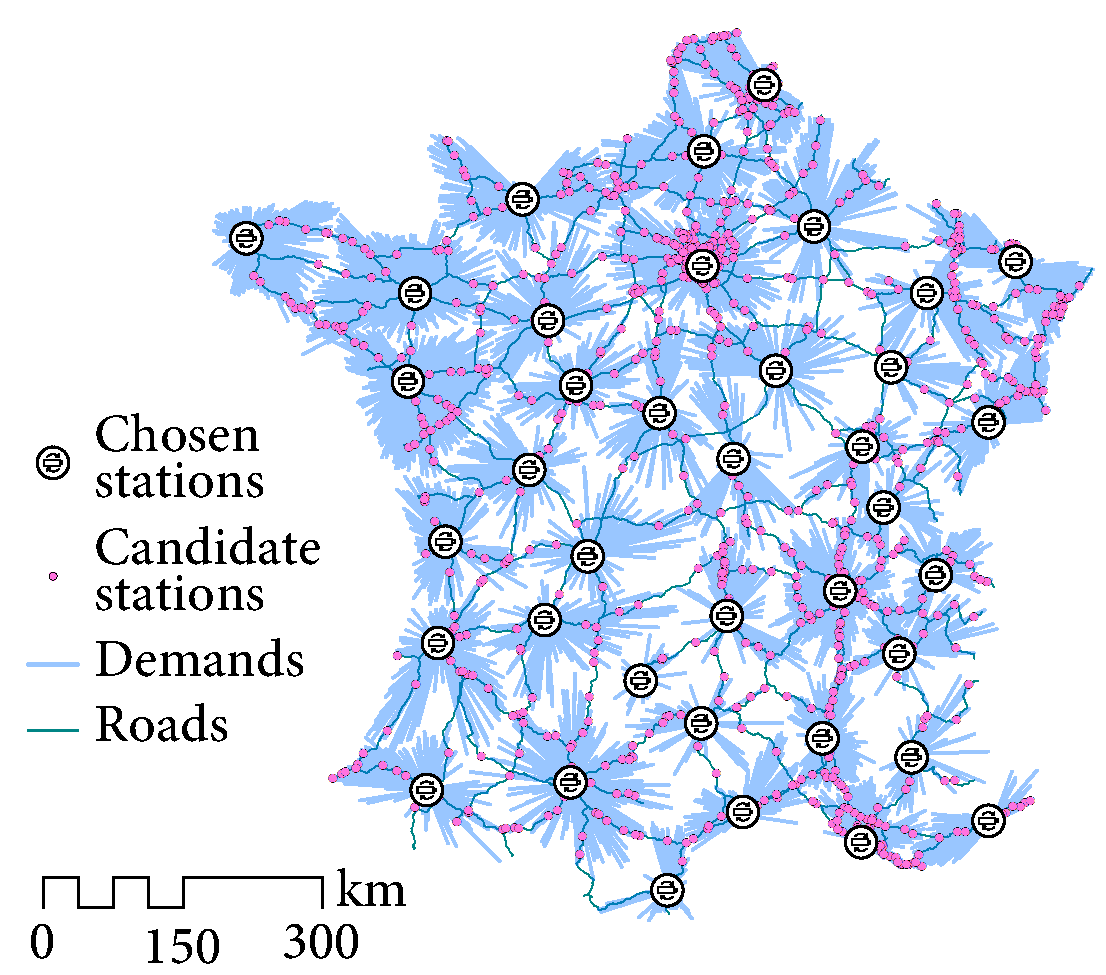
\includegraphics[width=\textwidth]{figures/France-allocation-charging-stations.pdf}
            % }
            \caption{Allocation of charging stations over the French road network. The big dots are the chosen stations, the little dots are the candidate stations, and the lines represent the allocated demands to the chosen stations.}
            \label{fig:France-location-allocation}
    \end{subfigure}%
    \quad %add desired spacing between images, e. g. ~, \quad, \qquad etc.
      %(or a blank line to force the subfigure onto a new line)
    \begin{subfigure}[t]{0.47\columnwidth}
            \centering
            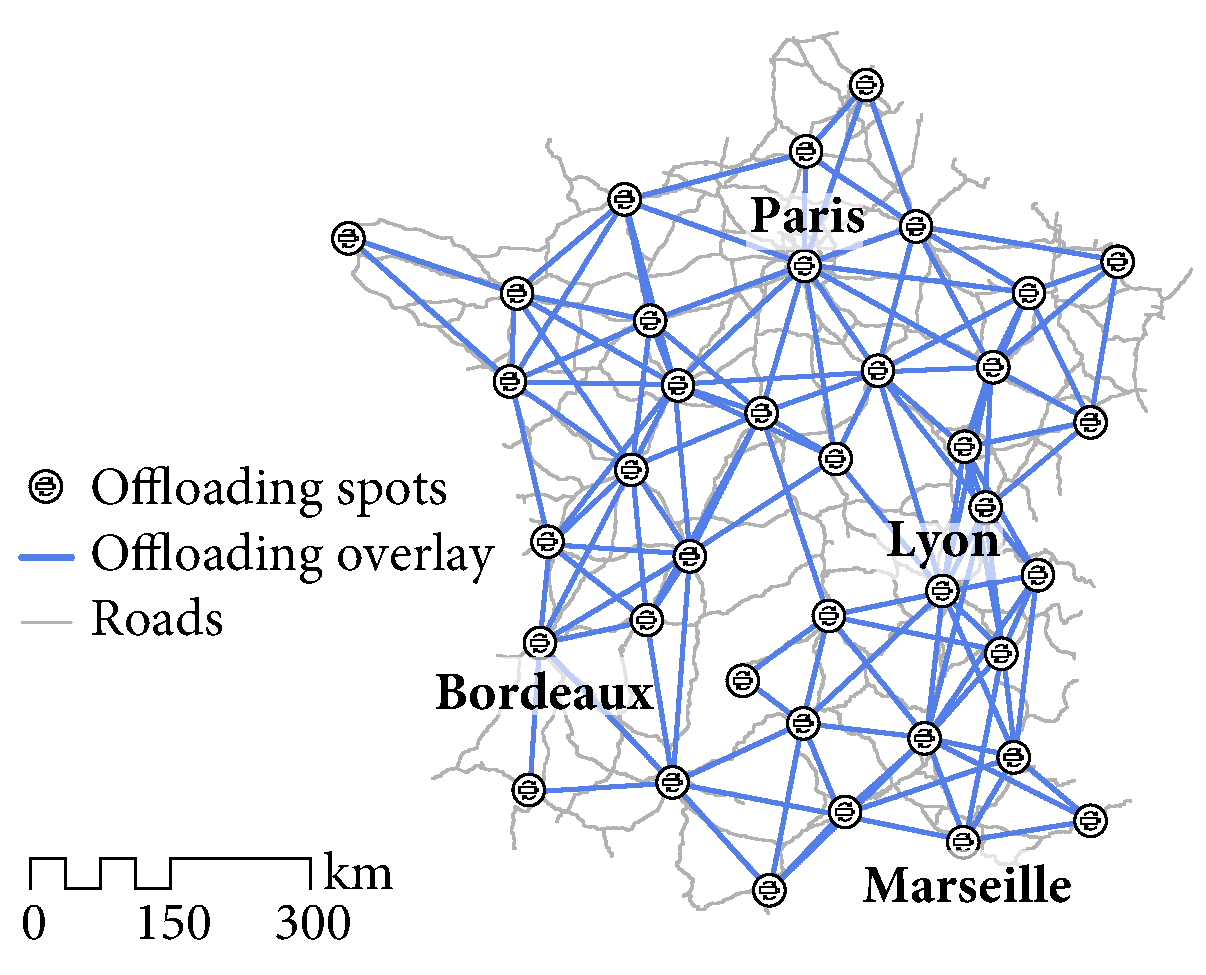
\includegraphics[width=\textwidth]{figures/France-overlay-wo-capacity.pdf}
            \caption{Resulting offloading overlay built on to of the road network of France. The offloading spots are those represented in Figure~\ref{fig:France-location-allocation}.}
            % (deduced from the AADT values)
            \label{fig:France-overlay-wo-capacity}
    \end{subfigure}
    \caption{Facility-allocation result and offloading overlay. The big dots are the chosen stations.}
\end{figure}

The facility-allocation algorithm selects the stations such that a maximum demand points are allocated to the charging stations within a range of 150~km, while minimizing the number of chosen stations. We assume that vehicle ownership is uniform throughout the territory~---~we can then weight the cities by their population. The chosen stations are allocated at most 150~km away from each other. This is enough for a vehicle with an autonomy of 300~km to reach the next closest station or return to the same station without depleting its battery. Finally, we assume that the stations have a capacity that suits the demand such that the waiting time is negligible. The waiting time is then restricted to the service time, which corresponds to the duration of the battery charge.

The resulting allocation outputs 38 stations scattered on the French road network, as shown in Fig.~\ref{fig:France-location-allocation}. We note that the stations are mainly allocated near major cities, as the demand from urban areas is higher than from rural areas.

\subsubsection{Complexity of the offloading overlay}
\label{sec:complexity-offloading-overlay}

The offloading overlay\index{offloading overlay} provides a logical view of the road network. Since the latter is very complex, it becomes quickly intractable to enumerate all the possible simple paths between two distant locations. The offloading overlay allows keeping some of the characteristics of the road network we need to perform our data transfer allocation problem, while reducing the complexity of the initial road network and making the path enumeration tractable. For this evaluation, we aim to show how the offloading overlay compares with the road network in terms of capacity. 

\begin{wrapfigure}[16]{o}[0.7\marginparwidth]{8cm}
    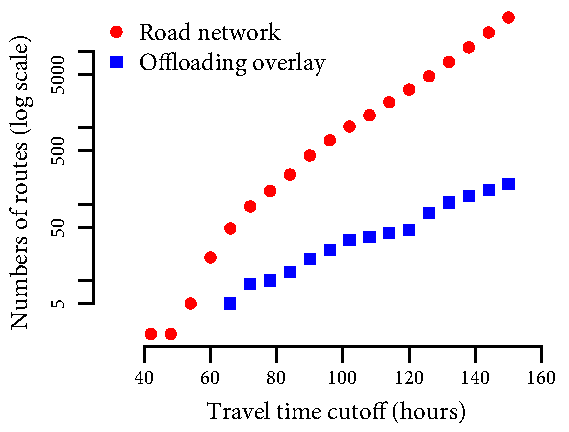
\includegraphics[width=7.5cm]{results/pathcount.pdf}
    \caption{Total number of simple paths in the road network and logical simple paths in the offloading overlay as a function of the travel time cutoff ($y$-axis is in a logarithmic scale).}
    \label{fig:pathcount}
\end{wrapfigure}
To this end, we instantiate an offloading overlay as defined in Section~\ref{sec:offloading-overlay-characterization}. We create it from the network of stations we planned to cover the main roads of France in the previous section. In the offloading overlay representation, the stations become the nodes of the offloading overlay, or offloading spots. The logical links between the stations correspond to the shortest route between two offloading spots. As noted before, we constrain the maximum length of the route to 300~km. The resulting offloading overlay is depicted in Figure~\ref{fig:France-overlay-wo-capacity}. Note that we do not need to fully characterize the logical links of the offloading overlay in terms of capacity to evaluate its benefits. We will fully characterize the logical links when conducting the evaluations in the following chapters.

We plotted the total number of simple paths bounded by a travel time cutoff in both the road network and the offloading overlay. The plot is represented in Figure~\ref{fig:pathcount} and shows the number of all simple paths as a function of the travel time cutoff of the enumerated paths. We note that, in both cases, the number of simple paths grows exponentially with the travel time cutoff. The number of simple paths is much larger on the road network compared to those enumerated in the offloading overlay. Also, the difference in the number of paths grows exponentially. This exponential growth is the main complexity factor to consider when solving the data transfer allocation problem.

\section{Discussions}
\label{sec:discuss}

\subsection{Drayage system}
As shown in Figure~\ref{fig:taxonomy}, data is offloaded from a conventional data network to the closest offloading spot using a drayage system\index{drayage|bb}. The drayage in our services is equivalent to the first and last mile of the access networks in an Internet-based transfer. The drayage can be carried out by different means:

\begin{itemize}
    
    \item \textit{Dedicated lines} (\eg optical fiber channels) can be set up between the different locations that need drayage. This solution would be adapted to connect locations that require continuous large data exchanges. However, it does not fit temporary data exchanges, as it is a costly solution (\eg the sources and destinations of a data transfer are only temporary). 

    \item \textit{Dedicated vehicles} can provide data drayage between the different locations. These vehicles would be equipped with storage and communication capabilities, with the data size and rates greater in magnitude than the common vehicles we consider in this thesis.

\end{itemize}


\subsection{Predicting the future direction of the stopping vehicles.}
For each stopping vehicle, the offloading spot must determine the subsequent offloading spot on the vehicle's route. The controller stores the previous locations of the vehicles in a historical database to help the offloading spots predict the remaining itinerary of the stopping vehicles. To this end, the controller can use probabilistic tools, such as Hidden Markov Models~\cite{simmons2006learning}, maximum entropy~\cite{ziebart2008maximum}, or Bayesian networks~\cite{liao2007learning,krumm2006predestination}. The partial trajectories of the vehicles can be known through the successive locations recorded by the navigation system of the vehicles. Note that, the current road traffic in the vicinity of the offloading spot can also help predict the most likely routes vehicles will take~\cite{xue2009traffic}.

\section{Conclusion}

In this chapter, we introduced the two tools that we will use in the following chapters to allocate the demands to offload data transfers on the road network. 

Firstly, we proposed a centralized architecture with a controller that has a holistic view of the system to manage and configure the offloading spots to match the requirements of demands to offload data. In the following chapters, we rely on this architecture to enable the efficient allocation and reliability of data transfers over the road network. We showed the benefits of the centralized architecture in the resulting throughput over a distributed architecture where the offloading spots take local forwarding decisions.

Secondly, we introduced the offloading overlay as a logical view used by the controller to represent the resources of the road network to mitigate its scale. The nodes of the overlay correspond to the offloading spots and the links characterize the movements of vehicles between the offloading spots as networking quantities relevant to the allocation of the data transfers, including the capacity, travel time, and data leakage. We showed that the offloading overlay effectively decreases the complexity of the main roads of France, as it provides a logical overlay with an exponential difference in the number of paths for given path travel times. 

In the next chapter, we will use both of these tools to assess the feasibility of the offloading service when comparing it to transfers on conventional data networks.